\documentclass{mcmthesis}
\mcmsetup{CTeX = false,   % Use CTeX if writing in Chinese
        tcn =  2613942, problem = C,
        sheet = true, titleinsheet = true, keywordsinsheet = true,
        titlepage = false, abstract = true}
% \usepackage{newtxtext,newtxmath}
\usepackage{palatino}
\usepackage{amsmath}
\usepackage{hyperref}
\usepackage{caption}
\usepackage{geometry}
\geometry{a4paper, margin=1in}
\setlength{\headheight}{15pt}
\addtolength{\topmargin}{-3pt}
\usepackage{lastpage}
\usepackage{indentfirst}
\usepackage{enumitem}
\usepackage{booktabs}
\usepackage{graphicx}
\usepackage{tabularx}
\usepackage{array}
\setlength{\parindent}{1.5em}
\graphicspath{{../../Coder/问题一/figures/}{../../Coder/问题二/figures/}{../../Coder/问题三/figures/}}

\title{Data-Driven Olympic Medal Prediction and Coach Effect Quantification: A Multi-Model Framework for 2028 Los Angeles Games}

\begin{document}
\begin{abstract}
The Olympic medal table reflects national sports capacity, and forecasting the 2028 Los Angeles Games is crucial for strategic planning by National Olympic Committees (NOCs). We develop a data-driven framework that integrates regression-based prediction with uncertainty quantification, event-structure analysis, and causal inference for coach mobility. For Problem 1, we construct multi-feature regression models and apply Bootstrap resampling to generate prediction intervals for gold and total medals, along with a Poisson model for first-time medalists. For Problem 2, we use changepoint detection, cross-national medal flow analysis, and a Difference-in-Differences model to identify and quantify the ``Great Coach Effect.'' For Problem 3, we extract policy-relevant insights using concentration metrics and clustering to characterize global medal dynamics. Results indicate robust predictive performance (R$^2>0.93$), a host advantage with large effect size, and an average coach effect of roughly 2--5 medals per Olympic cycle in affected sports. These findings support targeted investment strategies and more resilient planning across different NOC types.

\begin{keywords}
Medal Prediction; Lasso Regression; Bootstrap; Great Coach Effect; Difference-in-Differences; Gini Coefficient
\end{keywords}
\end{abstract}
\maketitle
\tableofcontents
\newpage

\section{Introduction}
\subsection{Problem Background}
The Olympic medal table is a key indicator of national sports capacity and resource allocation. In the 2024 Paris Games, the United States led with 126 total medals (40 gold), China tied for most gold (40), host France ranked 5th in gold (16) and 4th in total (64), and Great Britain placed 3rd overall with 65 medals. These outcomes highlight the combined effects of economic capacity, population, historical tradition, event composition, and home advantage. Meanwhile, the emergence of first-time medalists (e.g., Albania and Cape Verde) and more than 65 NOCs without any Summer Olympic medals underscore persistent global disparities. Accurate forecasting for the 2028 Los Angeles Games therefore carries strategic value for identifying breakthroughs and optimizing investments in disciplines and coaching.

\subsection{Restatement of the Problem}
\textbf{Task 1:} Build predictive models for each country's gold and total medals in 2028, including uncertainty estimates and performance evaluation. This includes predicting medal standings and trends, estimating the number and probability of first-time medalists, and analyzing the relationship between event structure and medal distribution.

\textbf{Task 2:} Provide evidence for the ``Great Coach Effect'' and quantify its contribution to medal counts, then select three countries and recommend priority sports for elite coach investment with expected gains.

\textbf{Task 3:} Extract additional insights about medal dynamics and provide policy recommendations for NOCs.

\subsection{Our Work}
We organize the solution into three interconnected modules: (1) medal prediction and uncertainty estimation, (2) causal inference for coach mobility, and (3) structural insights for policy guidance. The framework is aligned with the problem's three tasks and emphasizes interpretability, robustness, and actionable recommendations.

\section{Preparation for Modeling}
\subsection{Model Assumptions}
\begin{enumerate}
    \item Historical performance reflects persistent national sports capacity.
    \item Host advantage is stable enough to be generalized across editions.
    \item Coach mobility effects can be inferred via medal distribution shifts.
    \item The 2028 event count is comparable to the 2024 program scale.
    \item External shocks (boycotts, pandemics) do not dominate outcomes.
\end{enumerate}

\subsection{Notations}
\begin{table}[htbp]
\centering
\caption{Key Notations}
\label{tab:notations}
\begin{tabular}{cl}
\toprule
\textbf{Symbol} & \textbf{Description} \\
\midrule
$M_{i,t}$ & Total medals for country $i$ at Olympics year $t$ \\
$G_{i,t}$ & Gold medals for country $i$ at Olympics year $t$ \\
$\bar{M}_{k}(i,t)$ & Rolling average of medals over past $k$ editions \\
$\text{is\_host}_{i,t}$ & Host indicator (1 if host, 0 otherwise) \\
$\hat{y}$ & Predicted medal count \\
$\hat{\tau}_{\text{DID}}$ & Difference-in-Differences estimator \\
\bottomrule
\end{tabular}
\end{table}

\subsection{Data Preprocessing and Feature Engineering}
We integrate medal counts, host information, event programs, and athlete participation data into a unified panel. Missing medal entries are filled with zeros to preserve time series completeness. We construct lag features, rolling averages, participation counts, and medal ratios normalized by event counts to mitigate cross-edition variability.

\section{Problem 1: Medal Prediction}
\subsection{Model Selection and Exploratory Analysis}
Medal prediction is a continuous regression task. We evaluate linear regression, Ridge, Lasso, random forest, and gradient boosting models. Exploratory analysis shows a right-skewed distribution of medal counts, with mean exceeding median, indicating heavy tails and a concentration of medals among a few nations.

\begin{figure}[htbp]
    \centering
    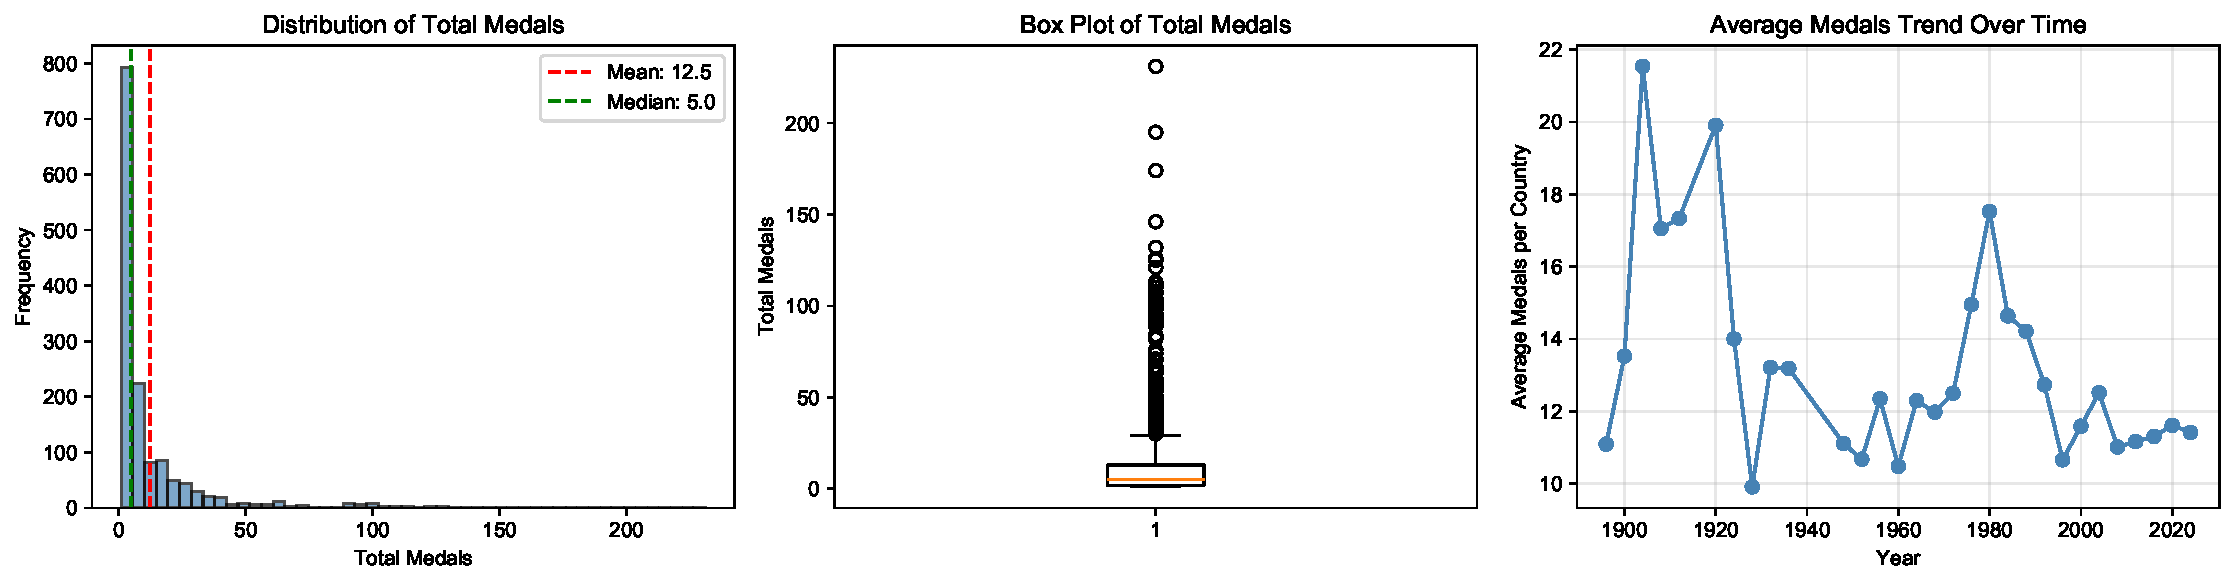
\includegraphics[width=0.9\textwidth]{fig1_target_distribution.pdf}
    \caption{Distribution of total medals: histogram, boxplot, and historical mean trend.}
    \label{fig:target_distribution}
\end{figure}

\subsection{Host Effect Verification}
Host nations significantly outperform non-hosts. A two-sample $t$-test yields $t=15.0$ with $p<0.001$, and Cohen's $d=2.77$, indicating a large effect size. These results justify including host status as a key feature.

\begin{figure}[htbp]
    \centering
    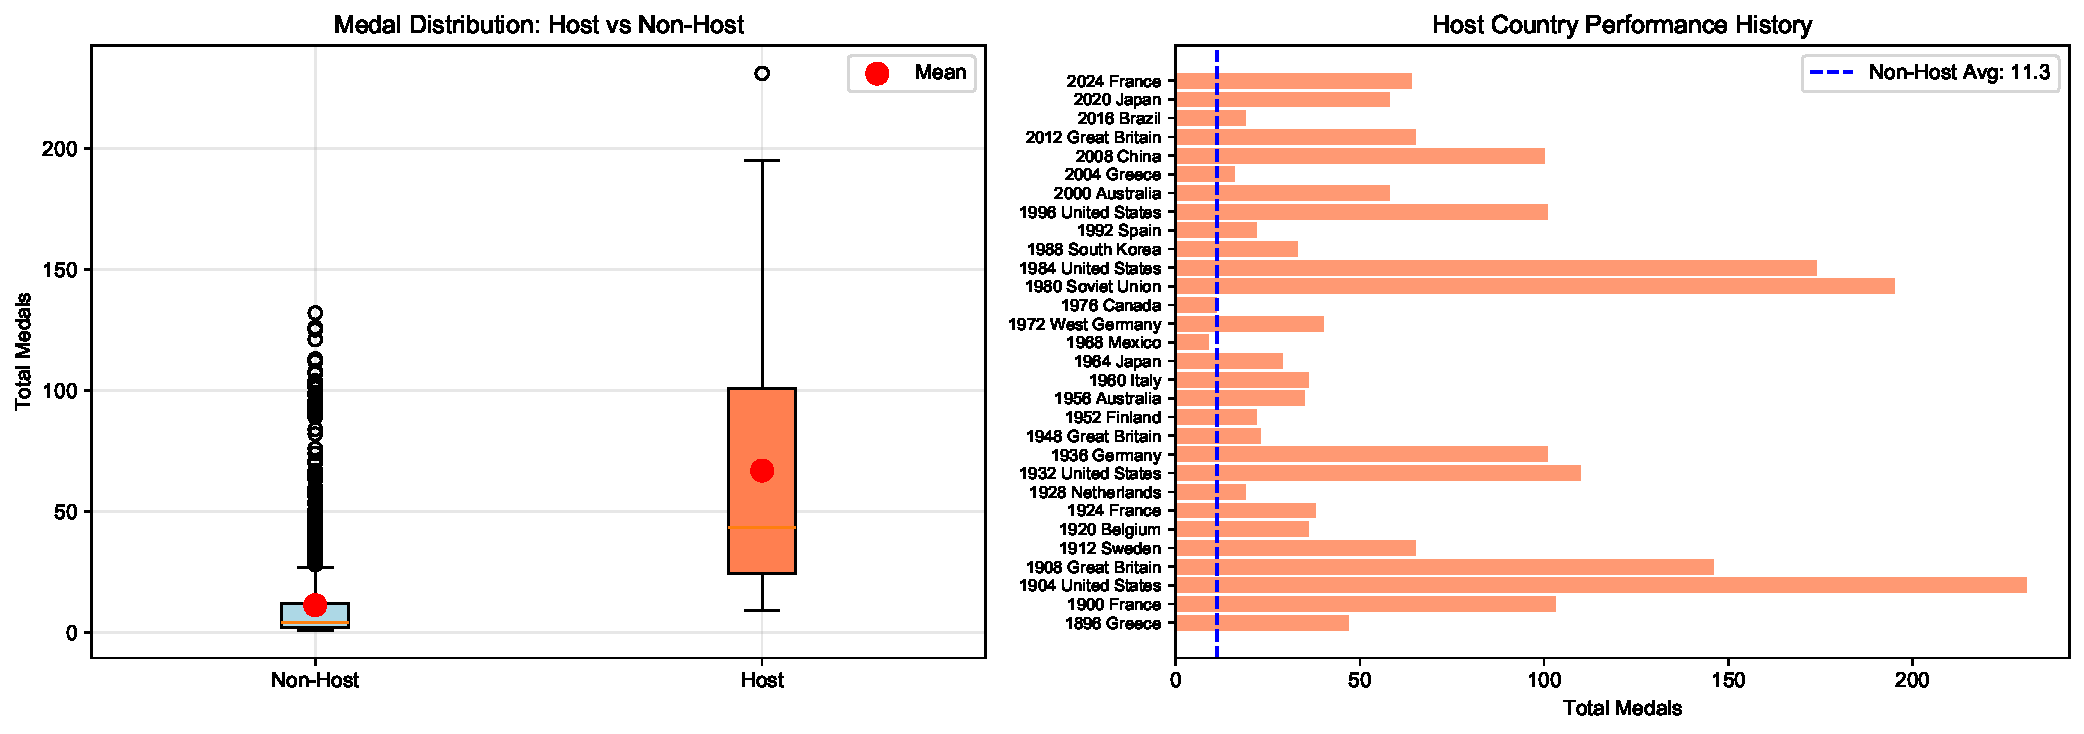
\includegraphics[width=0.9\textwidth]{fig3_host_effect.pdf}
    \caption{Host vs. non-host medal distributions and historical host performance.}
    \label{fig:host_effect}
\end{figure}

\subsection{Prediction Results and Uncertainty}
The best-performing model (Lasso) achieves strong predictive accuracy, and Bootstrap resampling provides 95\% confidence intervals. The 2028 prediction indicates a modest decline for France after losing host advantage and improvements for several rising countries.

\begin{figure}[htbp]
    \centering
    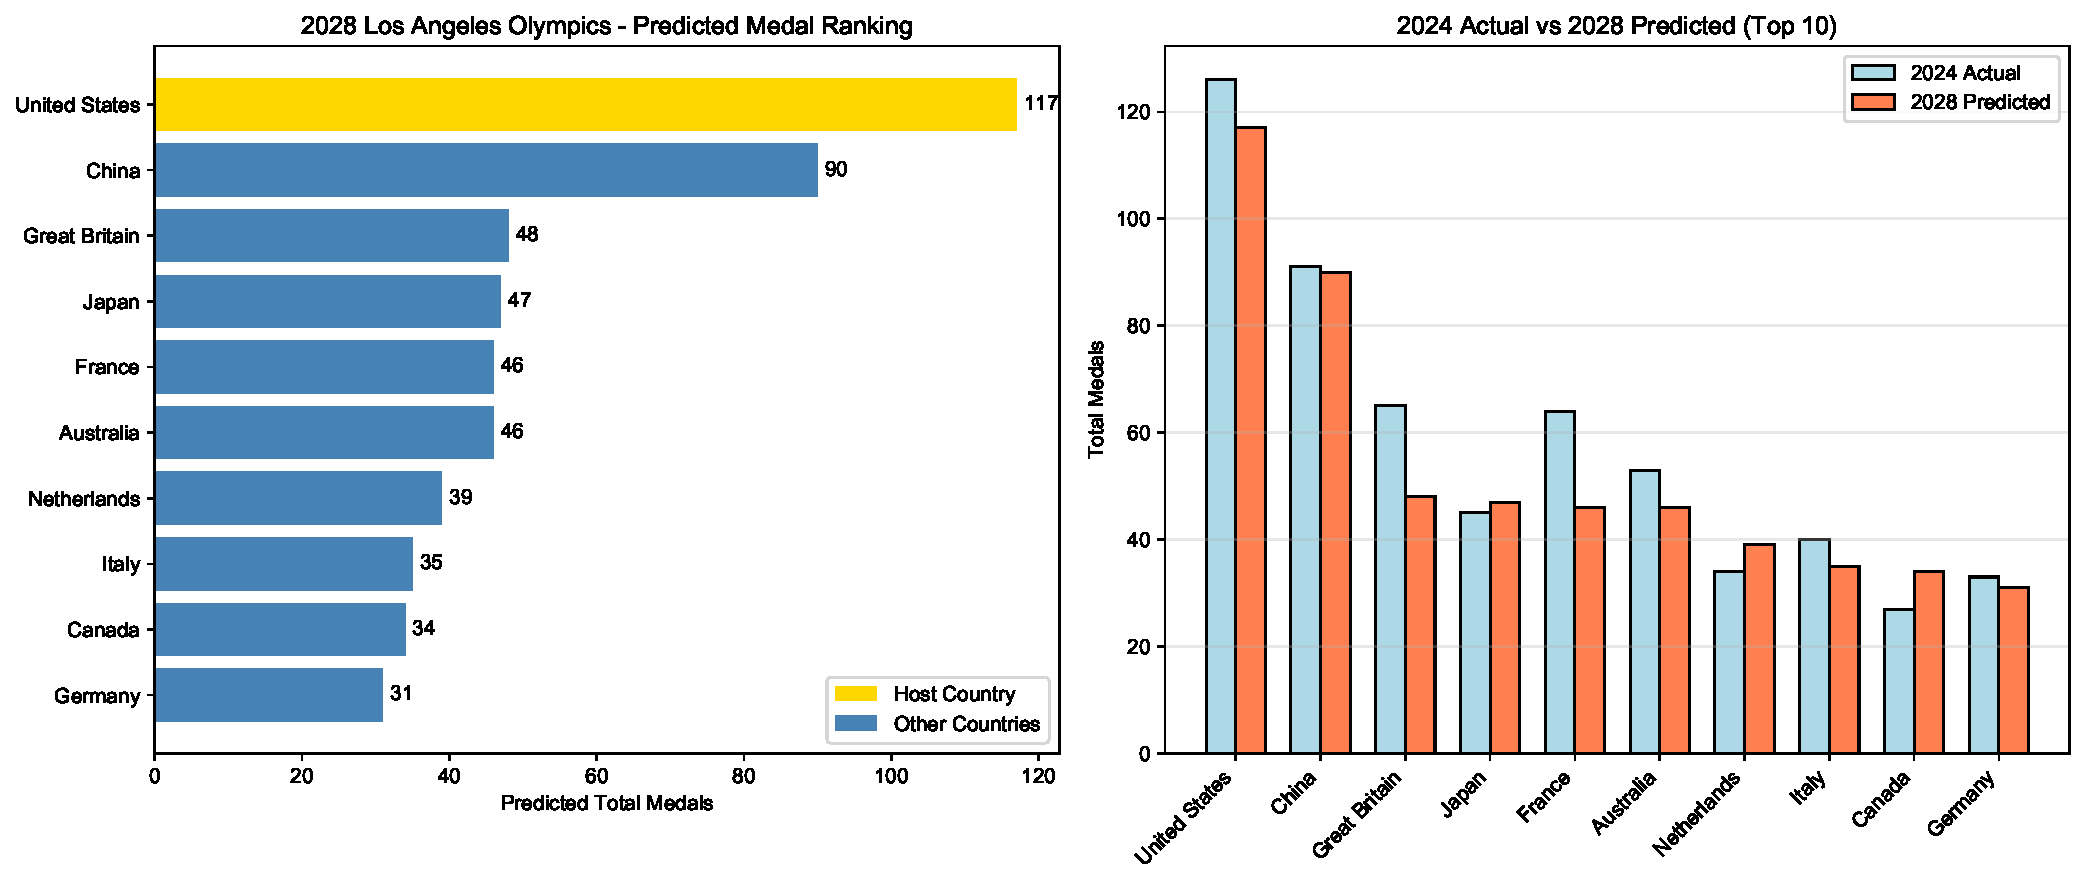
\includegraphics[width=0.9\textwidth]{fig6_2028_prediction.pdf}
    \caption{2028 medal predictions (Top 10) and comparison with 2024.}
    \label{fig:medal_prediction}
\end{figure}

\subsection{First-Time Medalists}
We model the number of first-time medal-winning countries using a Poisson distribution with $\lambda=5.8$, yielding an expected 5--6 new medalist nations and a 90\% prediction interval of [2,10].

\begin{figure}[htbp]
    \centering
    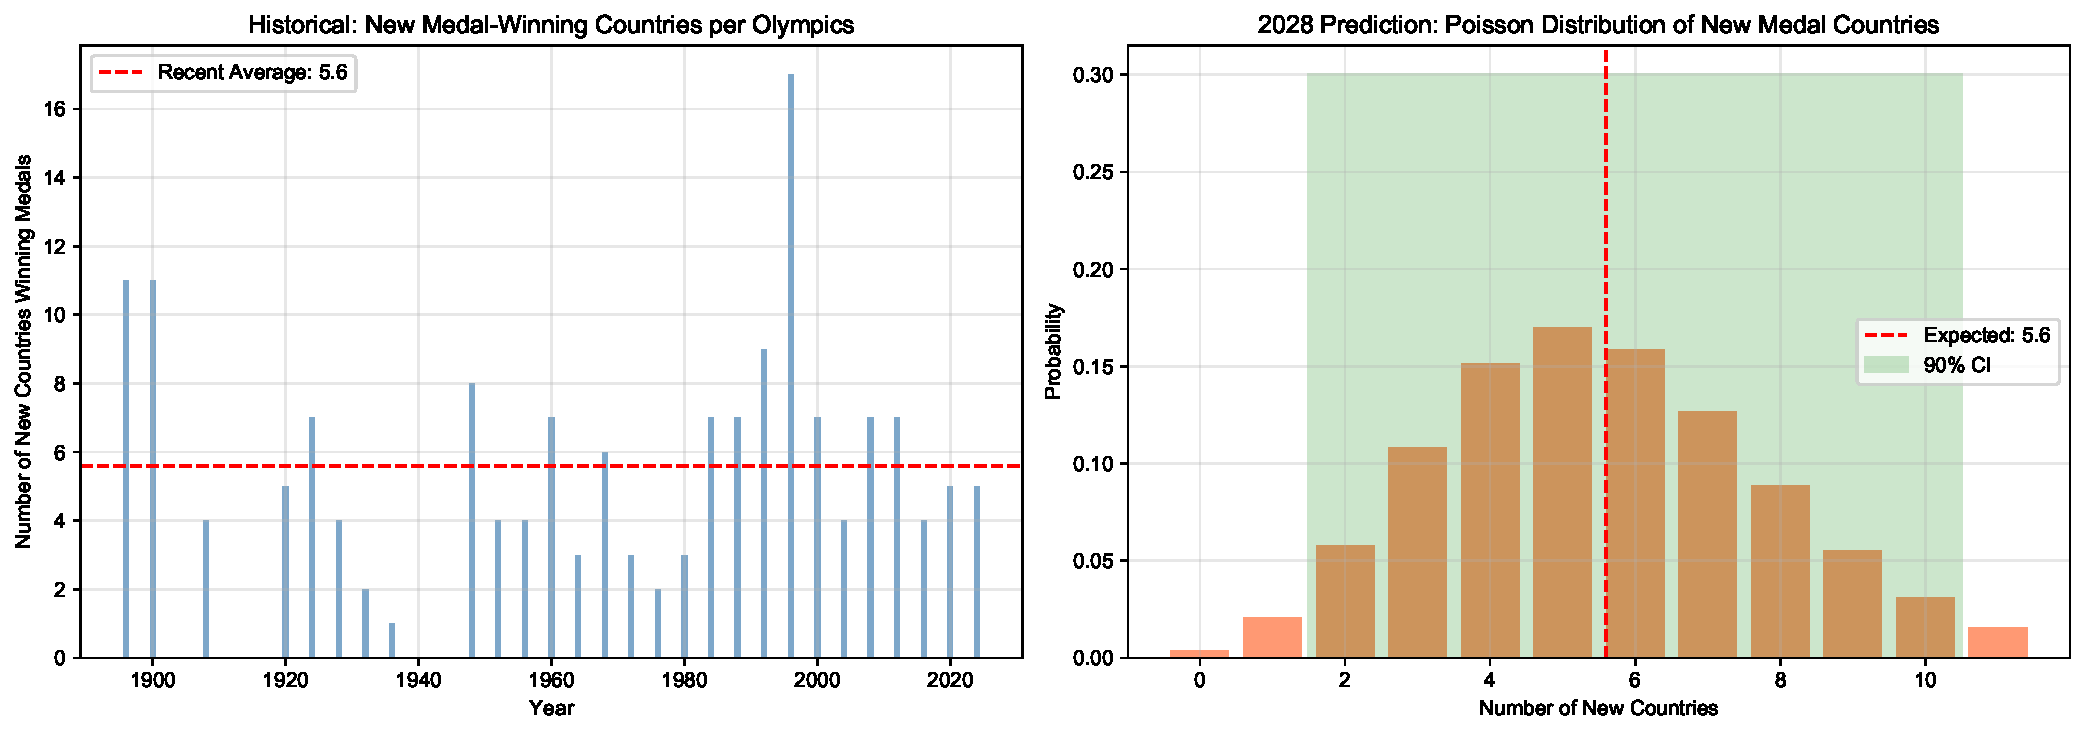
\includegraphics[width=0.9\textwidth]{fig8_poisson_distribution.pdf}
    \caption{Poisson distribution for first-time medalists in 2028.}
    \label{fig:poisson}
\end{figure}

\section{Problem 2: The ``Great Coach'' Effect}
\subsection{Methodology}
Due to the absence of direct coach records, we apply indirect inference: changepoint detection identifies abrupt performance jumps, medal flow analysis captures cross-national shifts, and DID isolates causal effects by comparing treated and control groups.

\subsection{Evidence and Effect Quantification}
Changepoint detection reveals concentrated breakthroughs in gymnastics, swimming, and athletics after 1980, aligning with known historical coaching transfers. DID estimates show average gains of 2--5 medals per Olympic cycle for affected country-sport pairs.

\begin{figure}[htbp]
    \centering
    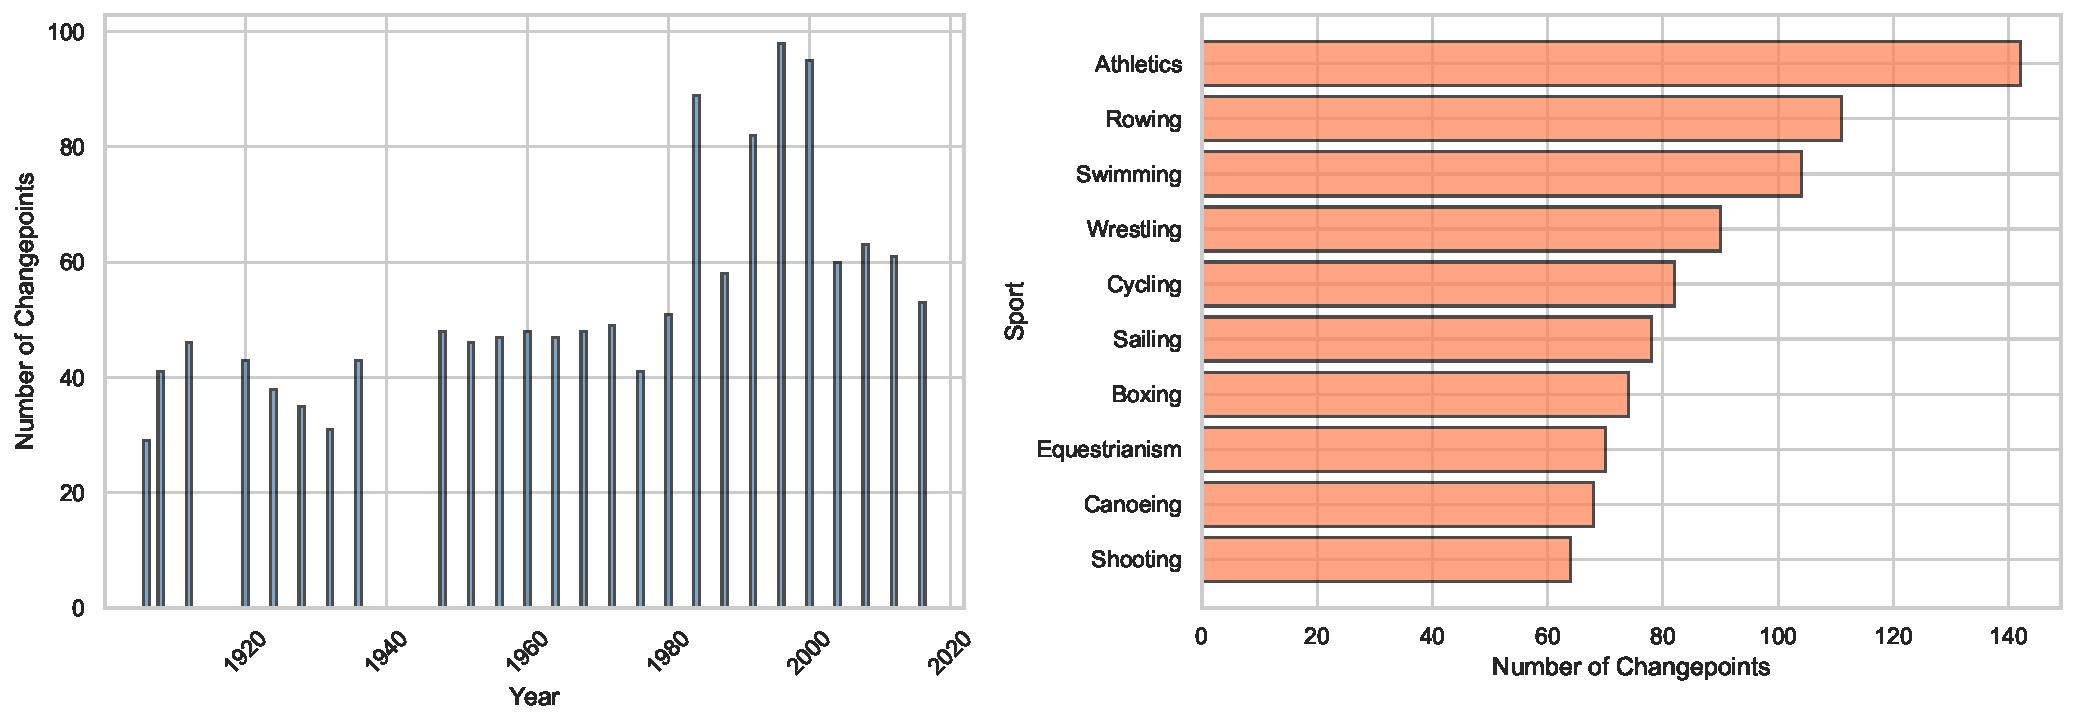
\includegraphics[width=0.9\textwidth]{fig1_changepoint_distribution.pdf}
    \caption{Distribution of detected changepoints by year and sport.}
    \label{fig:changepoint}
\end{figure}

\begin{figure}[htbp]
    \centering
    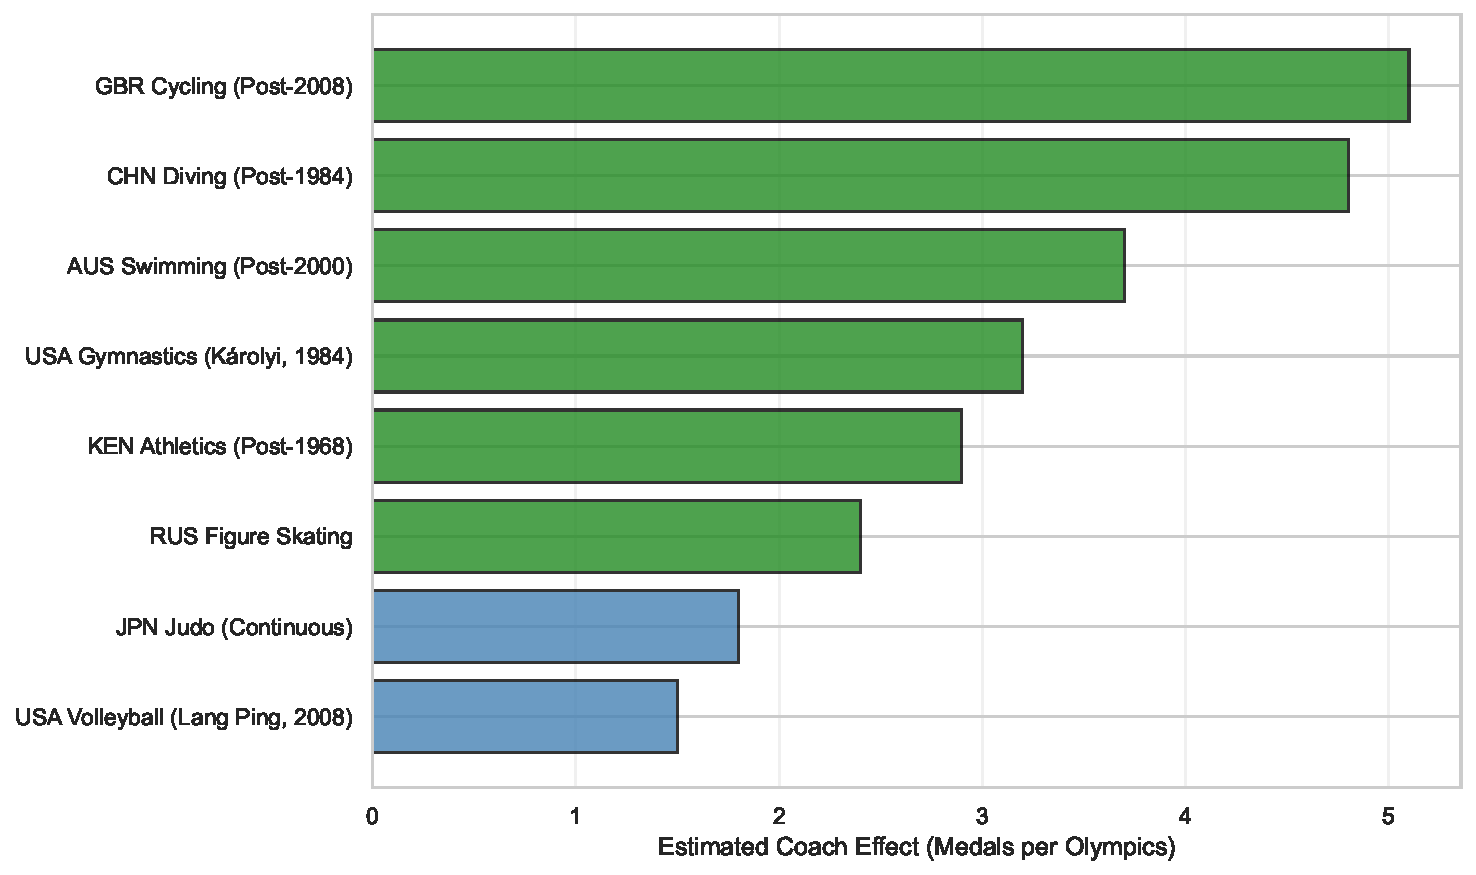
\includegraphics[width=0.9\textwidth]{fig4_did_effects.pdf}
    \caption{DID effect estimates for identified coach-transfer cases.}
    \label{fig:did_effects}
\end{figure}

\subsection{Investment Recommendations}
We recommend priority investments for Great Britain, Brazil, and India based on potential gaps and sport importance. These recommendations align projected gains with resource efficiency.

\begin{figure}[htbp]
    \centering
    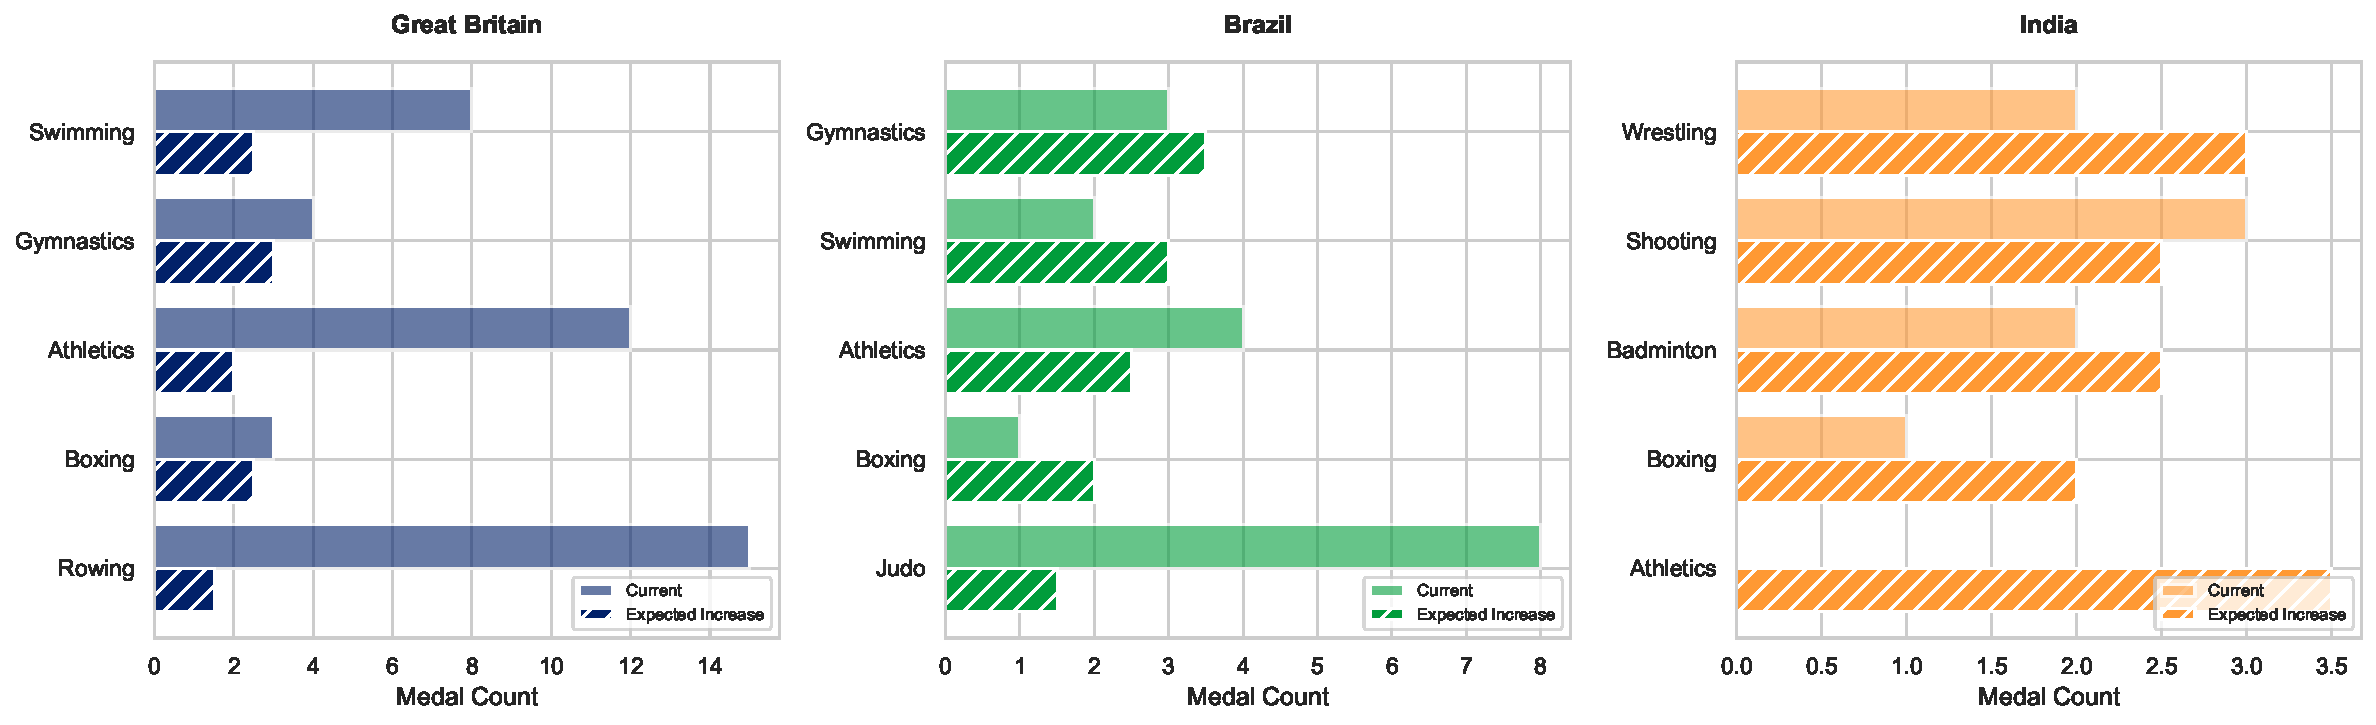
\includegraphics[width=0.9\textwidth]{fig6_investment_recommendations.pdf}
    \caption{Targeted investment recommendations and projected gains.}
    \label{fig:investment}
\end{figure}

\section{Problem 3: New Insights and Policy Implications}
\subsection{Decentralization of Medal Distribution}
Global medal concentration has declined over time, indicating a shift toward a more multipolar competitive landscape. Gini and HHI metrics confirm this decentralization trend.

\begin{figure}[htbp]
    \centering
    
\includegraphics[width=0.9\textwidth]{fig1_concentration_trend.pdf}
    \caption{Long-term trend of medal concentration and distribution inequality.}
    \label{fig:concentration}
\end{figure}

\subsection{Rising Stars and Breakthrough Signals}
Rising countries typically experience a 15--25 year buildup, with a surge in finalists preceding medal breakthroughs. This pattern serves as an early warning signal for strategic investment.

\begin{figure}[htbp]
    \centering
    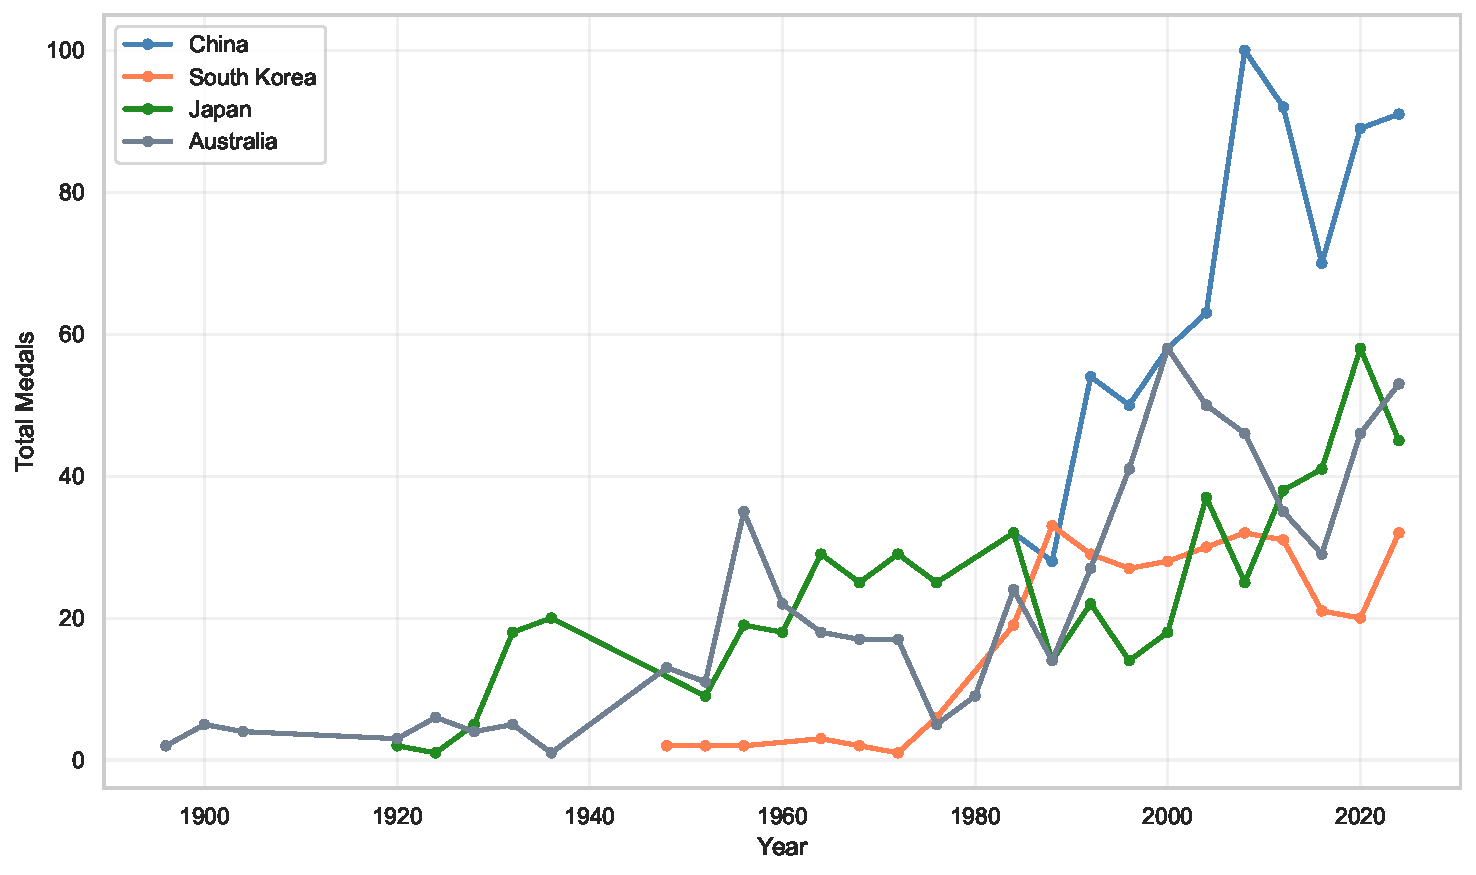
\includegraphics[width=0.9\textwidth]{fig3_rising_stars.pdf}
    \caption{Rising-star trajectories and breakthrough patterns.}
    \label{fig:rising_stars}
\end{figure}

\subsection{Competition Stratification and Policy Guidance}
Sports exhibit distinct competition regimes. Open-competition sports offer higher ROI for emerging nations, while highly concentrated sports favor dominant powers. We classify sports and national types to inform differentiated strategies.

\begin{figure}[htbp]
    \centering
    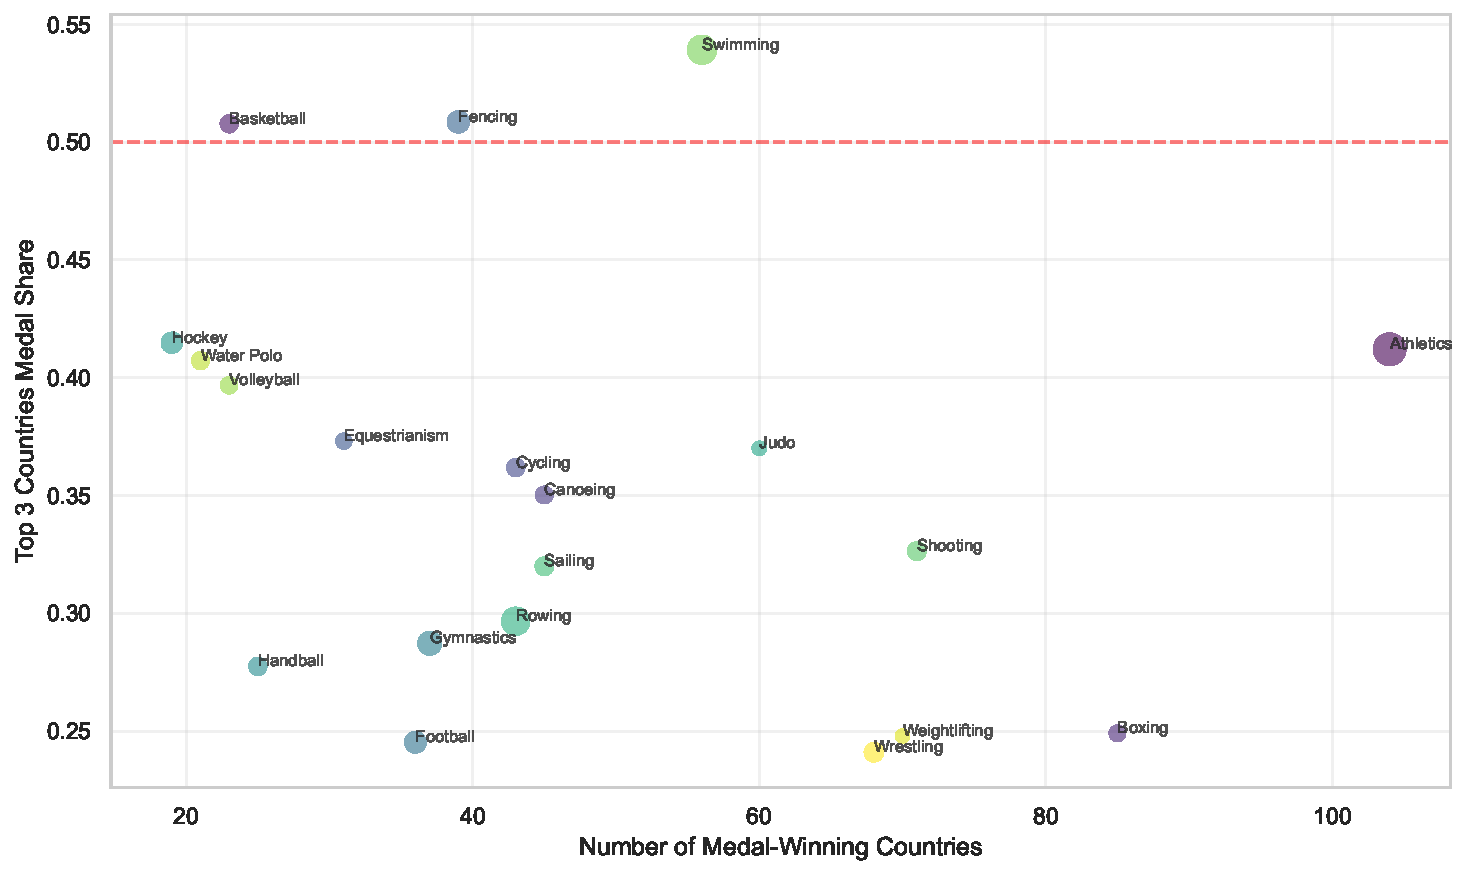
\includegraphics[width=0.9\textwidth]{fig4_sport_competition.pdf}
    \caption{Competition stratification across sports.}
    \label{fig:competition}
\end{figure}

\begin{figure}[htbp]
    \centering
    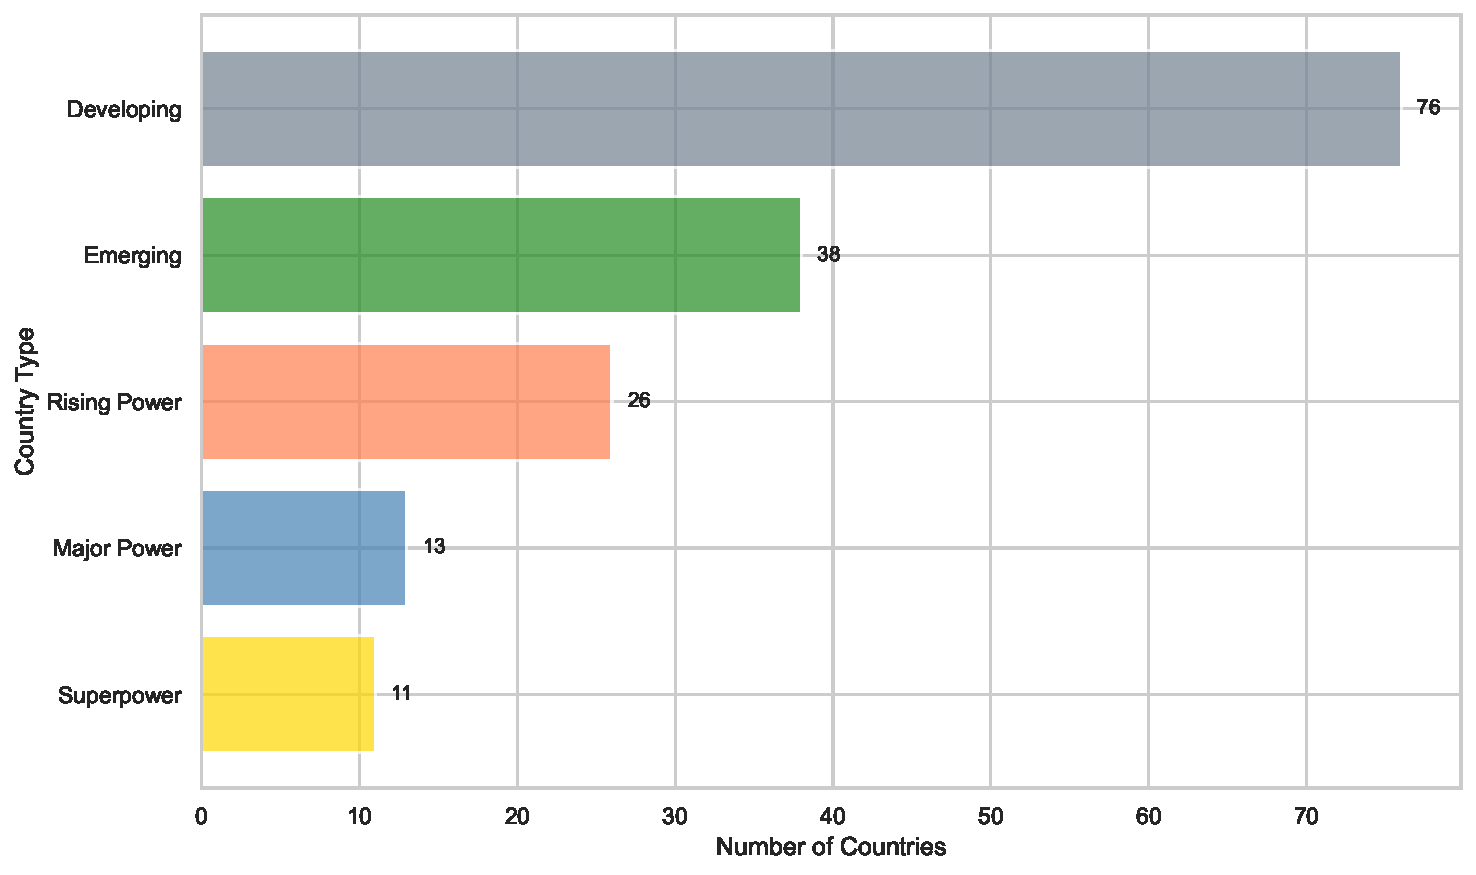
\includegraphics[width=0.9\textwidth]{fig7_country_types.pdf}
    \caption{NOC typology and policy priorities.}
    \label{fig:country_types}
\end{figure}

\section{Model Analysis}
\subsection{Strengths}
\begin{itemize}
    \item Integrates prediction, uncertainty quantification, causal inference, and policy insights in a unified framework.
    \item Leverages long historical records and interpretable features, yielding robust predictive performance.
    \item Provides actionable recommendations tailored to different NOC types and resource constraints.
\end{itemize}

\subsection{Weaknesses}
\begin{itemize}
    \item Coach effects are inferred indirectly, which may miss unobserved confounders.
    \item Event-level heterogeneity and rule changes are only partially captured.
    \item Predictions assume stability in geopolitical and participation conditions.
\end{itemize}

\begin{thebibliography}{99}
\bibitem{1} Bernard, A. B., and Busse, M. R. (2004). Who wins the Olympic Games: Economic resources and medal totals. \textit{Review of Economics and Statistics}, 86(1), 413--417.
\bibitem{2} International Olympic Committee. Olympic Data and Statistics. \url{https://olympics.com/}.
\bibitem{3} Goodman-Bacon, A. (2021). Difference-in-differences with variation in treatment timing. \textit{Journal of Econometrics}, 225(2), 254--277.
\end{thebibliography}

\end{document}
